\section{Création de prédicateurs}
\label{chap3.section1}
La création ou l'ingénieurie de prédicateurs (définis dans section \ref{chap2.section2}) est très généralement la toute première tâche d'un data scientist et l'une des plus longue. Dans ce domaine les données sont rarement utilisables sous leur forme brute pour entraîner des modèles d'apprentissage automatique car elles proviennent généralement de diverses bases de données et sont constituées de plusieurs tables (liées ou indépendantes) représentant différentes entités et leur relations. 

Ces données peuvent vite devenir extrêmement larges et complexes, dans les cas les plus
extrêmes une seule entité de la base de données pourrait avoir des dizaines d’enfants\footnote{Un enfant ici réfère à une entité qui a été créée par des opérations reproducibles éffectuées par ou sur une autre entité. Par exemple, dans un système de vente, une entité client pourrait avoir comme enfant une entité commande où l'entité commande contient toutes les commandes éffectuée par les différentes instances de l'entité client} qui
peuvent aussi avoir des enfants (donc des petits enfants pour l'entité de base). Sachant que la variable que l'on cherche à prédire est souvent une caractéristique de l'entité de base (comme la probabilité qu'un client revienne chez nous par exemple), ce genre de schéma complexifie le choix des prédicateurs puisqu'un prédicateur important peut être une caractéristique d'un enfant où d'un petit enfant (comme le nombre de commandes passées par le client ou le type de produits qu'il a commandé).

Avant de pouvoir créer des modèles de prédictions il est nécessaire de comprendre les
relations entre les différentes entités et les caractéristiques intrinsèques de l'entité elle
même pour en extraire des variables (\textit{features}) pouvant nous permettre de faire le lien entre le comportement des entitées et la variable qu’on souhaite prédire (\textit{target}).

Le langage des données peut être trivial des fois, par exemple supposons une table
contenant uniquement les heures de travail hebdomadaire de chaque employé d’une
entreprise. Un employé qui travaille plus est plus susceptible d’avoir une augmentation
ou une promotion par exemple, donc si l’on cherche à prédire quels employés auront des
promotions à la fin de l’année il est fort probable que cette information puisse nous aider,
nous avons donc déjà une variable indépendante pour prédire les promotions.

Maintenant supposons qu’au lieu de cette table assez simple nous possédons une table qui
contient les dates et les heures d’arrivées et de départs de chaque employé durant l’année.
C’est moins évident tout d’un coup, sur quoi devons nous entraîner le modèle et comment
représenter des dates et des heures? Même si on trouve une représentation optimale
(numérique) de ces variables, toutes ces variables sont-elles vraiment nécessaires pour
prédire qui aura une promotion à la fin de l’année? Elles répètent presque toutes la même
information sous différentes formes, on risquerait d’entraîner un modèle inutilement complexe et qui risque de se noyer dans le bruit et la redondance (ralentissant ou stoppant complètement l’apprentissage).

Pourtant les données sur les arrivées et les départs des employés dans les entreprises sont
typiquement plus fréquentes sous le deuxième format que le premier. En réalité, le
premier est forcément déduit du second. En effet, nous pouvons passer de cette deuxième table à la première juste en appliquant des opérations de transformations et d'agrégations pour par exemple passer du format “date et heure” à “heure” seulement ensuite soustraire les heures d'arrivées des heures de départs (pour avoir les heures de travail journalier), faire la moyenne de ces heures de travail journalier sur des périodes de sept jours (semaines) et enfin faire la moyenne de cette moyenne sur le nombre total de semaines travaillées pour avoir le nombre moyen d’heures travaillées par semaines au cours de l’année.

Ceci est un exemple plutôt simple illustrant un peu le processus général derrière de tâche
de création de prédicateurs permettant de passer des données brute aux features ou prédicateurs.

Ce travail est effectué par un ingénieur en données (Data Engineer) avant le processus de
création des modèles d’apprentissage. C’est une tâche fastidieuse dont la complexité
augmente souvent avec le nombre de tables (entités) et selon la profondeur des rélations (enfant, petits enfants, arrière petits enfants...) dans la base de données et qui requière
souvent une certaine expérience pour dénicher les meilleures features. Mais il s'agit aussi d'un travail qui devient vite extrêmement pénible quand l'ensemble de données brute que l'on possède dépasse une certaine taille et profondeur. L'ensembe de données avec lequel j'ai travaillé est constitué de \textbf{17 entités} dont l'entité de base (contenant des informations sur la demande de prêt et la variable à prédire) et 16 enfants de cette table de base. Certaines entités étaient tellement volumineuses qu'ils ont été obligés de les diviser en plusieurs tables, totalisant près de \textbf{70 tables} et \textbf{2588 colonnes} le tout regroupant des infomations tels que les demandes de prêt précedentes du client (s'il y'en a), son registre fiscal et d'autre informations personnelles et banquières sur les 1.526.659 démandeurs, certaines tables pouvant aller jusqu'à plus de 10 millions de lignes.

Alors je suis bien content qu'il n'y ait pas eu de petits enfants mais ça fait quand même une quantité colossal d'informations à analyser et à comprendre. Analyser toutes ces données afin de créer et évaluer des prédicateurs pertinents de façon manuelle me prendrait un temps énorme (risquerait d'aller jusqu'à un mois) or cette partie spécifique du flux de travail n'est pas ce qui nous intéresse le plus avec ce thème. Il me fallait trouver une solution beaucoup plus rapide, un moyen d'automatiser cette partie du travail.

\subsection{Création automatique de prédicateurs}
\label{chap3.sec1.sub1}
L'ingénieurie de prédicateurs est la partie du flux de travail qui nécéssite le plus l'intervention humaine donc les data scientist ont logiquement cherché à rendre ce travail moins long, surtout que la majeure partie du boulot consiste à écrire et modifier des fonctions pour appliquer les même calculs mathématiques à différentes table avec différents schémas. Il s'agissait de trouver un niveau d'abstraction qui s'approche au maximum de la compréhension humaine de cette tâche et qui puisse permettre la création d'algorithmes capable de prendre en charge ce processus.

Néanmoins, la création automatique de prédicateurs, faisant référence à des algorithmes capable de prendre en charge entièrement la création de prédicateur, est un concept plus ou moins récent dans le domaine de la science des données . Le concept fût d’abord formalisé par James Max Kanter et Kalyan Veeramachaneni dans leur papier de 2015 “Deep feature synthesis: Towards automating data science endeavors” où ils proposent un algorithme pour générer automatiquement des prédicateurs pour les ensembles de données relationnelles: c’est l’algorithme de Deep Feature Synthesis ou Synthèse approfondie des prédicateurs (\cite{kanter2015deep}).

L'algorithme suit les relations entre les différentes tables et une table de base, puis
applique séquentiellement des fonctions mathématiques d'aggrégation et de transformation le long de ces chemins, en fonction du type de données des colonnes (nombres, booléens, chaînes de caractères, horodatages etc...), pour enfin créer des prédicateurs. L’algorithme prend en entrée un ensemble interconnecté d’entités/tables.

Dans le papier, les auteurs ont décrit deux types de relations entre entités, les relations vers l'avant et les relations vers l'arrière (\textit{forward and backward relationships}), et trois types de prédicateurs pour une entité en fonction des relations qu'elle entretient avec d'autres entités: les prédicateurs d’entité (\textbf{efeat}), les prédicateurs directes (\textbf{dfeat}) et les prédicateurs relationnelles (\textbf{rfeat}).

Dans une relation vers l’avant, une instance d'une entité \(E^l\) est associée à une seule
instance d'une autre entité \(E^k\). Et une relation vers l'arrière est une relation qui lie une instance i dans \(E^k\) à toutes les instances m = {1 . . . M} dans \(E^l\) qui ont une relation vers l’avant avec k. L’exemple trivial est celui d’une relation “parent-enfants” où un enfant n’a basiquement qu’un parent alors que le parent peut avoir beaucoup d’enfants. D’ailleurs les scientifiques ont majoritairement adopté cette appellation.

\begin{enumerate}
    \item Les prédicateurs d'entité (efeat): ce sont les caractéristiques directes de l'entité (les variable dans la table de base de l'entité) comme le sexe, l’âge, le revenu, etc... En fonction de la variable à prédire, ce type feature pourrait même être utilisé directement comme prédicateurs. On peut aussi leur appliquer des transformations, par exemple: calculer l'âge à partir de la date de naissance.
    \item Les prédicateurs directes (dfeat): les prédicateurs directes sont appliquées sur les relations vers l’avant (Enfant -> Parent). Dans ceux-ci, des features de l’entité i ∈ \(E^k\) (enfant) sont directement transférées sous forme de caractéristiques pour l'entité j ∈  \(E^l\) (parent). Un exemple pourrait être le prix d'un produit qui devient un attribut dans la table des commandes.
    \item Les prédicateurs relationnelles (rfeat): les prédicateurs relationnelles sont appliquées aux relations vers l'arrière (Parent -> Enfants). Ils sont dérivés pour une instance i de l'entité \(E^k\) en appliquant une fonction mathématique à \(x_{:,j|ek=i}^l\), qui est une collection de valeurs pour une caractéristique j dans l’entité \(E^l\) assemblée en extrayant toutes les valeurs de j dans l'entité \(E^l\) où l'identifiant de \(E^k\) est \(ek = i\). Cette transformation est donnée par la formule \(x_{i,j’}^k = rfeat(x_{:,j|ek=i}^l)\). Quelques exemples de fonctions rfeat sont min (pour trouver le minimun d'un ensemble de valeur), max (pour trouver le maximumn d'un ensemble de valeur) et count (pour compter les apparitions d'une valeur en particulier).
\end{enumerate}

Avec ce niveau d'abstraction, le but de l'algorithme de Deep Feature Synthesis est de trouver et de calculer les dfeats et les rfeats pour une entité cible \(E^k\), les ajoutez à la table \(E^k\) et calculez les efeats sur l'ensemble. Dans le cas où une entité enfant de l’entité cible possède ses propres enfants, nous pouvons générer les prédicateurs de manière récursive en utilisant la même séquence décrite ci-dessus. La récursion peut se terminer lorsque l'on atteint une certaine profondeur (eg, arrière petits enfants) ou s'il n’y a plus d’enfants.

Ainsi Kanter et Veeramachaneni ont proposé et implémenté un algorithme qui possède un niveau d'abstraction suffisant pour imiter l'intuition humaine pour la tâche de création de prédicateurs. La figure \ref{fig:fig2} apporte une illustration de l’algorithme

\begin{figure}
    \centering
    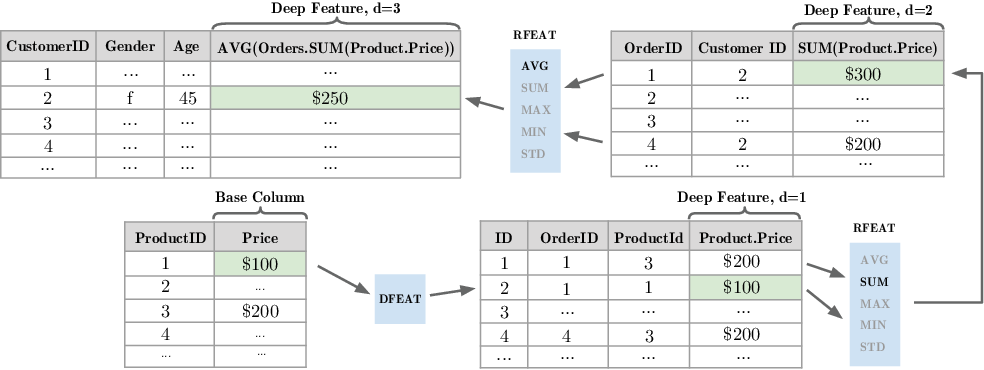
\includegraphics[width=0.75\linewidth]{images/Fig4DFS.png}
    \caption{Visualisation d'une itération de la Synthèse approfondie de prédicateurs (DFS)}
    \label{fig:fig2}
\end{figure}

\subsection{Implémentation}
\label{chap3.sec1.sub2}
J'ai donc utilisé l'agorithme de Synthèse approfondie de prédicateurs sur les données fournies par Home Credit Group. Pour cela j’ai utilisé le langage de programmation python et deux bibliothèques entre autres que j'aimerai souligner: \textbf{“featuretools”} qui
offre une implémentation de DFS et \textbf{"Dask"} pour paralléliser les calculs (\cite{dask2016dask}).

Au vue de la taille de l’ensemble de données fournit par Home Credit j’ai été obligé d’implémenter quelques autres stratégies, notamment pour partitionner les données, car trop volumineuse pour pouvoir être procédé directement même avec 30 Go de mémoire vive. L'ensemble de données a donc été partitionnée de manière à ce que chaque partition contienne exactement 17 tables (1 entité == 1 table) avec toutes les informations nécéssaires pour faire la synthèse des prédicateurs pour un sous ensemble de maximum 12.000 exemples (demandeurs). Résultant en 128 partitions de 17 tables parfaitement indépendantes (les partitions sont indépendantes entre elles mais les tables dans la même partition sont liées).

L'utilisation de Dask pour paralléliser les opérations a permit d'appliquer DFS sur plusieurs partitions en même temps (4 pour être précis, correspondant au nombre de cœurs du processeur) et donc calculer plusieurs matrices de prédicateurs simultanément, diminuant le temps d'exécution du code de 44-50 heures à approximativement 24 heures. Le code en question est librement accessible sur Kaggle et github (\cite{diarra2024autofeatureengineering}).